\documentclass{beamer}
\usepackage[utf8]{inputenc}
\usepackage[english]{babel}
\usepackage{helvet}
\usepackage[T1]{fontenc}
\usepackage[inline]{asymptote}
\usepackage{asy_helper}
\usepackage{slide_helper}
\usepackage{tikz}
\usetikzlibrary{shapes.geometric, arrows}
\usepackage{pgfplots}
\pgfplotsset{compat=1.5} 
\usepgfplotslibrary{statistics}
\usetikzlibrary{external}
\tikzexternalize%

\title[MA205 - Section 4.2]{Geometric Distribution}

\newcommand{\prob}[1]{P\left({#1}\right)}
\newcommand{\jointprob}[3]{\prob{{#1}~\text{#2}~{#3}}}
\newcommand{\condprob}[2]{\prob{{#1}~|~{#2}}}
\newcommand{\comb}[2]{_{#1}C_{#2}}

\begin{document}
\begin{frame}
\titlepage
\end{frame}

\begin{frame}
  \begin{definition}
    When an individual trial only has two possible outcomes, often labeled \texttt{success} or \texttt{failure}, it is called a \textbf{Bernoulli random variable}.
  \end{definition}\pause

  \begin{note}
    It does not matter which outcome is labeled as \texttt{success} or \texttt{failure}, just that there are only two outcomes.
  \end{note}\pause

  \begin{note}
    Bernoulli random variables are often denoted with
    \begin{itemize}
    \item 1 for \texttt{success}
    \item 0 for \texttt{failure}
    \end{itemize}
  \end{note}\pause

  \begin{note}
    The events \texttt{success} and \texttt{failure} are complements.
  \end{note}
\end{frame}

\begin{frame}
  \begin{example}\label{universal donor}
    \vspace{-2mm}
    Subjects are randomly selected for the National Health and Nutrition Examination Survey conducted by the National Center for Health Statistics, Centers for Disease Control and Prevention.\pause
    
    \vspace{1mm}
    A person is a universal donor if they have group O and type Rh blood.\pause
    
    \vspace{1mm}
    If we think of each subject as a trial then:\pause
    \begin{itemize}
    \item If a person is a universal donor, we label them a \texttt{success}.\pause
    \item If a person is not a universal donor, we label them a \texttt{failure}.
    \end{itemize}\pause

    If there is a 6\% chance that a person is a universal donor, then:\pause
    \begin{itemize}
    \item The probability of a success is $p=0.06$\pause
    \item The probability of a failure is $q=1-p=\pause 0.94$
    \end{itemize}
  \end{example}\pause

  \begin{note}
    \texttt{success} and \texttt{failure} are not moral descriptions. We could have just as easily labeled the universal donors as \texttt{failure}.
  \end{note}
\end{frame}

\begin{frame}
  \begin{definition}
    The \textbf{sample proportion}, $\hat{p}$, is the sample mean:
    \begin{equation*}
      \begin{aligned}
        \hat{p} = \dfrac{\text{\# of successes}}{\text{\# of trials}}
      \end{aligned}
    \end{equation*}
  \end{definition}\pause

  \begin{example}
    Suppose we observe the ten trials of a Bernoulli random variable:
    \begin{equation*}
      \begin{aligned}
        1~1~1~0~1~0~0~1~1~0
      \end{aligned}
    \end{equation*}\pause
    The sample proportion of these observations would be:
    \begin{equation*}
      \begin{aligned}
        \hat{p} = \dfrac{1+1+1+0+1+0+0+1+1+0}{10}\pause = 0.6
      \end{aligned}
    \end{equation*}
  \end{example}
\end{frame}

\begin{frame}
  \begin{block}{Bernoulli Random Variable}
    If $X$ is a random variable that takes value 1 with probability $p$ and 0 with probability $q=1-p$, then $X$ is a Bernoulli random variable with mean and standard deviation:

    \vspace{-4mm}
    \begin{equation*}
      \begin{aligned}
        \mu=p
        \qquad
        \sigma=\sqrt{p(1-p)}
      \end{aligned}
    \end{equation*}
  \end{block}\pause

  \begin{example}
    In Example~\ref{universal donor}, $X$ describes the chances a subject is a universal donor, with probability of success $p=0.06$.\pause

    \vspace{1mm}
    The mean of $X$ is:
    \begin{equation*}
      \begin{aligned}
        \mu=p\pause
        =0.06\pause
      \end{aligned}
    \end{equation*}
    The standard deviation of $X$ is:
    \begin{equation*}
      \begin{aligned}
        \sigma = \sqrt{p(1-p)}\pause
        =\sqrt{0.06(1-0.06)}\pause
        =\sqrt{0.0564}\pause
        =0.237486842
      \end{aligned}
    \end{equation*}
  \end{example}
\end{frame}

\begin{frame}
  \begin{definition}
    The \textbf{geometric distribution} is used to describe how many trials it takes to observe a success.
  \end{definition}\pause

  \begin{example}
    If we are looking for universal donors as in Example~\ref{universal donor}, then the probability the first universal donor found is the first persion is $0.06$.\pause

    \vspace{1mm}
    The probability that the first universal donor is the second person.

    \vspace{-6mm}
    \begin{equation*}
      \begin{aligned}
        \jointprob{1^{\text{st}}~\text{no}}{and}{2^{\text{nd}}~\text{yes}} = (1-0.06)(0.06) = (0.94)(0.06) = 0.0564
      \end{aligned}
    \end{equation*}\pause

    \vspace{-6mm}
    The probability that the first universal donor is the third person.

    \vspace{-6mm}
    \begin{equation*}
      \begin{aligned}
        \jointprob{1^{\text{st}}~\text{no}~\text{and}~2^{\text{nd}}~\text{no}}{and}{3^{\text{rd}}~\text{yes}} = (0.94)(0.94)(0.06) = 0.053016
      \end{aligned}
    \end{equation*}\pause

    \vspace{-6mm}
    The probability that the first universal donor is the $n^{\text{th}}$ person.

    \vspace{-6mm}
    \begin{equation*}
      \begin{aligned}
        \jointprob{1^{\text{st}}~\text{through}~{(n-1)}^{\text{th}}~\text{no}}{and}{n^{\text{th}}~\text{yes}} &= (0.94)\cdots(0.94)(0.06)\\
        &= {(0.94)}^{n-1}\cdot0.06
      \end{aligned}
    \end{equation*}
  \end{example}
\end{frame}

\begin{frame}
  \begin{block}{Geometric Distribution}
    If the probability of a success in one trial is $p$ and the probability of failure is $1-p$, then the probability of finding the first success in the ${n}^{\text{th}}$ trial is given by
    \begin{equation*}
      \begin{aligned}
        {(1-p)}^{n-1}\cdot p
      \end{aligned}
    \end{equation*}
    The mean, variance and standard deviation of this wait time are
    \begin{equation*}
      \begin{array}{lll}
        \mu=\dfrac{1}{p} &
        \sigma^2=\dfrac{1-p}{p^2} &
        \sigma=\sqrt{\dfrac{1-p}{p^2}}
      \end{array}
    \end{equation*}
  \end{block}\pause

  \begin{note}
    The trials need to be both independent and identical to use the geometric distribution.
  \end{note}
\end{frame}

\begin{frame}
  \begin{example}
    The geometric distribution for $p=0.7$ 
    \begin{center}
      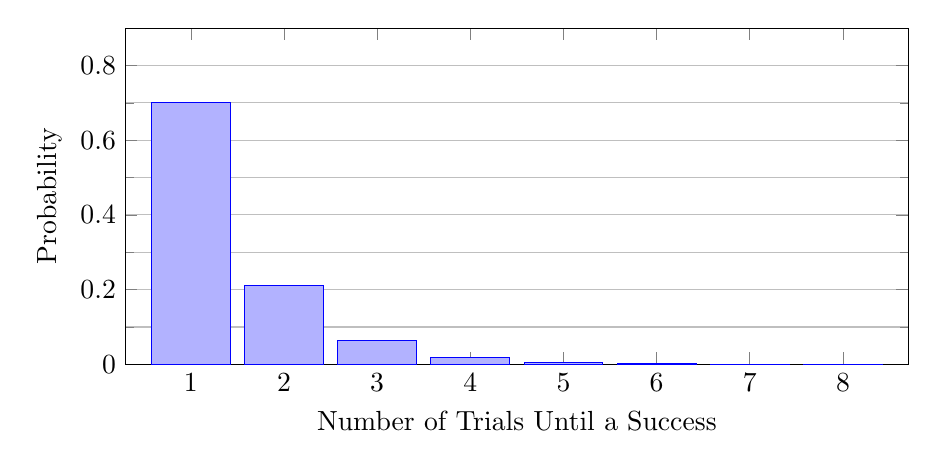
\begin{tikzpicture}
        \begin{axis}[
            height=5.85cm,
            width=0.95\textwidth,
            enlarge x limits=0.1,
            ymajorgrids=true,
            minor y tick num=1,
            yminorgrids=true,
            ylabel={Probability},
            xlabel={Number of Trials Until a Success},
            bar width=1cm,
            ybar stacked,
            ymin=0,
            ymax=0.9,
            ytick={0,0.2,...,1},
            xtick=data,
            legend style={fill=legend, fill opacity=1},
          ]
          \addplot+
          coordinates
          {
            (1, .7)
            (2, 0.21)
            (3, 0.063)
            (4, 0.0189)
            (5, 0.00567)
            (6, 0.001701)
            (7, 0.00051)
            (8, 0.000153)
          };
        \end{axis}
      \end{tikzpicture}
    \end{center}
  \end{example}\pause

  \begin{note}
    We call this the geometric distribution because the probabilities decrease exponentially fast as $n$ increases.
  \end{note}
\end{frame}

\begin{frame}
  \begin{note}
    The expected value, $\mu$, tells us, on average, how many trials it takes to get a success. The higher $p$, the fewer it takes.
  \end{note}\pause
  
  \begin{example}
    Since the probability of someone being a universal donor is $p=0.06$, the expected value is:

    \vspace{-3mm}
    \begin{equation*}
      \begin{aligned}
        \mu = \dfrac{1}{p}\pause
        = \dfrac{1}{0.06}\pause
        = 16.666666667
      \end{aligned}
    \end{equation*}\pause

    \vspace{-4mm}
    It should take, on average, 16.7 people until a universal donor is found.
  \end{example}\pause

  \begin{example}
    The probability of getting a \textquote{heads} on a fair coin is $p=0.5$, so the expected value is:

    \vspace{-3mm}
    \begin{equation*}
      \begin{aligned}
        \mu = \dfrac{1}{p}\pause
        = \dfrac{1}{0.5}\pause
        = 2
      \end{aligned}
    \end{equation*}\pause

    \vspace{-4mm}
    On average, it should only take two flips to get a \textquote{heads}.
  \end{example}
\end{frame}

\begin{frame}
  \begin{example}
    The probability that a universal donor is in the first three trials is:\pause

    \vspace{-5mm}
    \begin{equation*}
      \begin{aligned}
        \prob{\text{first or second or third}}
        &= \prob{\text{first}} + \prob{\text{second}} + \prob{\text{third}} \\\pause
        &= {(1-.06)}^{1-1}\cdot0.06 + {(1-.06)}^{2-1}\cdot0.06\\\pause
        &\hspace{3.62cm} + {(1-.06)}^{3-1}\cdot0.06 \\\pause
        &= 0.169416
      \end{aligned}
    \end{equation*}

    \vspace{-2mm}
    There is roughly a 16.9\% chance a universal donor will be one of the first three people.
  \end{example}\pause

  \begin{note}
    We could have also used complements:

    \vspace{-2mm}
    \begin{equation*}
      \begin{aligned}
        \prob{\text{first or second or third}}
        &= 1 - \prob{\text{none in first three}} \\\pause
        &= 1 - {(1-0.06)}^3 \\\pause
        &= 0.169416
      \end{aligned}
    \end{equation*}
  \end{note}
\end{frame}
\end{document}
